% ------------------------------------------------------------------------------
% TYPO3 Version 10.0 - What's New (English Version)
%
% @author	Michael Schams <schams.net>
% @license	Creative Commons BY-NC-SA 3.0
% @link		http://typo3.org/download/release-notes/whats-new/
% @language	English
% ------------------------------------------------------------------------------

\section{Änderungen für Integratoren}
\begin{frame}[fragile]
	\frametitle{Änderungen für Integratoren}

	\begin{center}\huge{Kapitel 3:}\end{center}
	\begin{center}\huge{\color{typo3darkgrey}\textbf{Änderungen für Integratoren}}\end{center}

\end{frame}

% ------------------------------------------------------------------------------
% TYPO3 Version 10.0 - Breaking Changes

\begin{frame}[fragile]
	\frametitle{Änderungen für Integratoren}
	\framesubtitle{Breaking Changes}

	\small
		Hinweis für Integratoren: Einige PHP-Code-, TSconfig-, TypoScript-Optionen
		und -Bedingungen sowie Scheduler-Aufgaben wurden als veraltet markiert.

		\vspace{0.2cm}

		Entsprechend der \textbf{Deprecation} von TYPO3 wurden diese 
		Komponenten in TYPO3 v10.0 geändert oder entfernt.

		Aktivieren Sie das Verfallsprotokoll, testen Sie Ihren Code sorgfältig und überprüfen
		Sie das Protokoll, um mögliche Probleme zu ermitteln. Verwenden Sie den integrierten
		\href{https://docs.typo3.org/m/typo3/reference-coreapi/master/en-us/ApiOverview/ExtensionScanner/Index.html}{Extension Scanner}
		um einen vollständigen Bericht über Inkompatibilitäten von Extensions zu erhalten.

	\normalsize

\end{frame}

% ------------------------------------------------------------------------------
% Feature | 78432 | Add log message for Switch User action

\begin{frame}[fragile]
	\frametitle{Änderungen für Integratoren}
	\framesubtitle{Backend User Switch}

	\begin{itemize}
		\item Eine Log-Nachricht wird erstellt, wenn ein Administrator zu einem anderen Backend-Benutzer wechselt:
	\end{itemize}

	\begin{figure}
		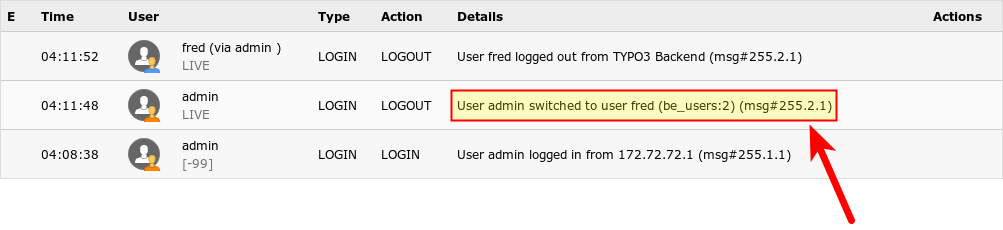
\includegraphics[width=0.90\linewidth]{ChangesForIntegrators/78432-SwitchUserActionLogMessage.png}
	\end{figure}

\end{frame}

% ------------------------------------------------------------------------------
% Feature | 83734 | Add support for current page in configcache
% Breaking | 88564 | PageTSconfig setting TSFE.constants removed
% Breaking | 88657 | Popup configuration in FormEngine dropped

\begin{frame}[fragile]
	\frametitle{Änderungen für Integratoren}
	\framesubtitle{TypoScript Changes}

	\begin{itemize}
		\item Die TypoScript-Eigenschaft \texttt{config.cache}  unterstützt jetzt das Stichwort
			"\texttt{current}" um auf die aktuelle Seite zu verweisen. Zum Beispiel:\newline
			\smaller\texttt{config.cache.all = fe\_users:current}\normalsize

		\item Die Seiten/User TSconfig-Einstellung \texttt{TSFE.constants} wurde entfernt.

			\begin{itemize}\smaller
				\item[\ding{228}]Fügen Sie die TypoScript-Bedingungen in Setup/Constants ein und definieren Sie eine ordentliche Konfiguration in der Datei \texttt{ext\_localconf.php}.
			\end{itemize}

		\item Die folgenden zwei Optionen zum Konfigurieren der Größe von Popup-Fenstern wurden entfernt:

			\begin{itemize}
				\item \texttt{options.popupWindowSize}
				\item \texttt{options.rte.popupWindowSize}
			\end{itemize}

	\end{itemize}

\end{frame}

% ------------------------------------------------------------------------------
% Breaking | 88640 | Database field sys_template.nextLevel and TypoScript sublevel inheritance removed
% Task | 88755 | Remove POST option from typolink.addQueryString

\begin{frame}[fragile]
	\frametitle{Änderungen für Integratoren}
	\framesubtitle{TypoScript-Änderungen}

	\begin{itemize}
		\item Das Datenbankfeld \texttt{nextLevel} der Datenbanktabelle
			\texttt{sys\_template} wurde entfernt.

			\begin{itemize}\smaller
				\item[\ding{228}] Ersetzen Sie den Datensatz (die UID ist im Feld \texttt{nextLevel}) durch eine Bedingung zum Hinzufügen von TypoScript für Unterseiten gespeichert. Zum Beispiel: \texttt{[tree.level > 1]}
			\end{itemize}\normalsize

		\item Folgende Werte sind \textbf{nicht erlaubt}:

			\begin{itemize}\smaller
				\item \texttt{typolink.addQueryString.method = POST}
				\item \texttt{typolink.addQueryString.method = GET,POST}
				\item \texttt{typolink.addQueryString.method = POST,GET}
			\end{itemize}\normalsize

			\begin{itemize}\smaller
				\item[\ding{228}] Ändern Sie die Zuweisungen in TypoScript, Fluid und PHP.
			\end{itemize}\normalsize

	\end{itemize}

\end{frame}

% ------------------------------------------------------------------------------
% Breaking | 87583 | Remove obsolete APC Cache Backend implementation
% Breaking | 87558 | Consolidate extbase caches

\begin{frame}[fragile]
	\frametitle{Änderungen für Integratoren}
	\framesubtitle{Caches}

	% decrease font size for code listing
	\lstset{basicstyle=\tiny\ttfamily}

	\begin{itemize}
		\item Das Caching-Framework unterstützt das \texttt{ApcBackend} nicht mehr

			\begin{itemize}\smaller
				\item[\ding{228}] Verwenden Sie stattdessen \textbf{APCu}  - beachten Sie das "u".
			\end{itemize}

\begin{lstlisting}
OLD:
$GLOBALS['TYPO3_CONF_VARS']['SYS']['caching']['cacheConfigurations']['rootline']['backend'] =
\TYPO3\CMS\Core\Cache\Backend\ApcBackend::class;

NOW:
$GLOBALS['TYPO3_CONF_VARS']['SYS']['caching']['cacheConfigurations']['rootline']['backend'] =
\TYPO3\CMS\Core\Cache\Backend\ApcuBackend::class;
\end{lstlisting}

		\item Die Extbase-Caches \texttt{extbase\_reflection} und \texttt{extbase\_datamapfactory\_datamap}
			wurden konsolidiert und sind jetzt als einzelner Cache unter dem Namen "\texttt{extbase}" verfügbar.

	\end{itemize}

\end{frame}

% ------------------------------------------------------------------------------
% Breaking | 87009 | Use multiple translation files by default in EXT:form

\begin{frame}[fragile]
	\frametitle{Änderungen für Integratoren}
	\framesubtitle{Formular-Framework}

	% decrease font size for code listing
	\lstset{basicstyle=\tiny\ttfamily}

	\begin{itemize}
		\item Die folgende Option wurde umbenannt:\newline
			\small\texttt{translationFile} \textrightarrow\hspace{0.1cm}\texttt{translationFiles}\normalsize
		\item Die Standardübersetzungsdateien sind jetzt bei Index 10 registriert:

			\begin{itemize}
				\item \texttt{EXT:form/Resources/Private/Language/locallang.xlf}
				\item \texttt{EXT:form/Resources/Private/Language/Database.xlf}
			\end{itemize}

		\item Die benutzerdefinierten YAML-Konfigurationsdateien müssen aktulisiert werden.

\begin{lstlisting}
OLD:
translationFile: path/to/locallang.xlf

NEW:
translationFiles:
  20: path/to/locallang.xlf
\end{lstlisting}

	\end{itemize}

\end{frame}

% ------------------------------------------------------------------------------
% xxxxx | Cache Storage Type

\begin{frame}[fragile]
	\frametitle{Änderungen für Integratoren}
	\framesubtitle{Cache Speichertyp(1)}

	\begin{itemize}

		\item TYPO3 verfügt über ein flexibles Caching-System mit einer Standardkonfiguration,
			die für die meisten Anwendungsfälle ideal ist.
		\item Der Speichertyp kann jetzt konfiguriert werden, um die Caches zu optimieren und die Leistung
			je nach individueller Umgebung zu steigern.

			\begin{itemize}
				\item Wählen Sie den \textbf{Datenbank} Speicher für eine Standardumgebung
					oder wenn beispielsweise ein Netzwerkdateisystem (NFS) verwendet wird.
				\item Wählen Sie das \textbf{Dateisystem} wenn beispielsweise eine verteilte Datenbank 
					eingerichtet wird.
				\item Verwenden Sie \textbf{custom cache settings}, um den Speicher für
					jeden Cachetyp einzeln zu konfigurieren.
			\end{itemize}

		\item Bei komplexeren Installationensollten speicherbasierte Caches wie zum Beispiel
			\href{https://redis.io/}{Redis}
			oder
			\href{https://memcached.org/}{Memcached}
			berücksichtigt werden.

	\end{itemize}

\end{frame}

% ------------------------------------------------------------------------------
% xxxxx | Cache Storage Type

\begin{frame}[fragile]
	\frametitle{Änderungen für Integratoren}
	\framesubtitle{Cache Speichertyp (2)}

	\begin{itemize}

		\item Backend: \textbf{WARTUNG} \ding{223}\hspace{0.1cm}\textbf{Einstellungen} \ding{223}\hspace{0.1cm}\textbf{Cache}:
		\end{itemize}

	\begin{figure}
		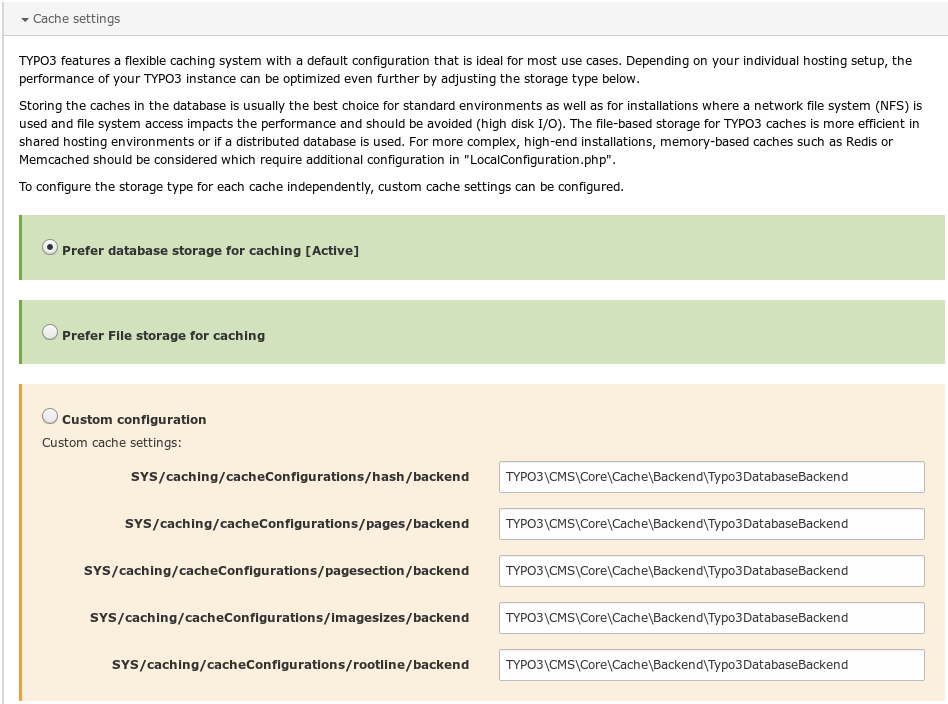
\includegraphics[width=0.60\linewidth]{ChangesForIntegrators/xxxxx-CacheStorageType.png}
	\end{figure}

\end{frame}

% ------------------------------------------------------------------------------
% 87499 | Drop extensions "taskcenter" and "sys_action" from core

\begin{frame}[fragile]
	\frametitle{Änderungen für Integratoren}
	\framesubtitle{Task-Center und \texttt{EXT:sys\_action}}

	\begin{itemize}

		\item Die Erweiterungen \texttt{EXT:taskcenter} and \texttt{EXT:sys\_action}
			wurden aus dem Core entfernt.

		\item Sie sind jetzt als separate Erweiterungen in der
			\href{https://extensions.typo3.org/}{TER}
			oder
			\href{https://github.com/FriendsOfTYPO3}{GitHub} verfügbar.

		\item Behalten Sie die 
			\href{https://typo3.org/community/teams/typo3-development/initiatives/typo3-dashboard-initiative/}{Dashboard Initiative}
			 im Auge, um einen neuen und viel besseren Lösungsansatz zu finden.

	\end{itemize}

\end{frame}

% ------------------------------------------------------------------------------
% Feature | 88648 | Define Twitter Card Type In Page Properties
% Important | 86577 | Query parameters are now included in canonicalized URLs

\begin{frame}[fragile]
	\frametitle{Änderungen für Integratoren}
	\framesubtitle{Sonstiges}

	% decrease font size for code listing
	\lstset{basicstyle=\tiny\ttfamily}

	\begin{itemize}

		\item Der Typ einer Twitter-Karte kann nun ausgewählt/konfiguriert werden.
			Diese Option gibt das Metatag \texttt{twitter:card} im Frontend aus.

\begin{lstlisting}
page {
  meta {
    twitter:card = summary_large_image
    twitter:card.replace = 1
  }
}
\end{lstlisting}

		\item In kanonisierten URLs sind standardmäßig nur Parameter enthalten, die zur Berechnung des cHash erforderlich sind.
			Zusätzliche Abfrageparameter können folgenderweise konfiguriert werden:

\begin{lstlisting}
$GLOBALS['TYPO3_CONF_VARS']['FE']['additionalCanonicalizedUrlParameters'].
\end{lstlisting}

		\smaller
			Hinweis: Fügen Sie nur Parameter hinzu, die den Inhalt Ihrer Seite ändern, damit die Suchmaschinen  den Inhalt Ihrer Seite nicht als doppelten Inhalt klassifizieren.
		\normalsize

	\end{itemize}

\end{frame}

% ------------------------------------------------------------------------------
% Breaking | 88681 | Import Of PHP Files In Import Export Files Removed
% Breaking | 88500 | RTE image handling functionality dropped
% Breaking | 81950 | Remove leftover workspaces unpublishing functionality

\begin{frame}[fragile]
	\frametitle{Änderungen für Integratoren}
	\framesubtitle{Sonstiges}

	% decrease font size for code listing
	\lstset{basicstyle=\tiny\ttfamily}

	\begin{itemize}

		\item beim Importieren von XML-Daten mit \texttt{EXT:impexp} gilt jetzt das File-Deny-Muster und 
			eingebettete PHP-Dateien werden abgelehnt.

		\item Die RTE-Bildbearbeitungsfunktion wurde vollständig entfernt.
			Verwenden Sie z.B. für die Image-Unterstützung in CKEditor 
			\texttt{EXT:rte\_ckeditor\_image}.

		\item Eine Eigenschaft zum \textit{Unpublishing} von Datensätzen in Workspaces wurde in v10 entfernt
			(einschließlich des Datenbankfelds \texttt{sys\_workspace.unpublish\_time}). Diese Funktion wurde in TYPO3 v4.5 deaktiviert und wurde nicht vom TYPO3-Core verwendet oder bereitgestellt.

	\end{itemize}

\end{frame}

% ------------------------------------------------------------------------------
% Breaking | 88772 | JavaScript script tags omit type=text/javascript in HTML5
% Remove system extension EXT:rsaauth
% Remove system extension EXT:fe_edit

\begin{frame}[fragile]
	\frametitle{Änderungen für Integratoren}
	\framesubtitle{Sonstiges}

	% decrease font size for code listing
	\lstset{basicstyle=\tiny\ttfamily}

	\begin{itemize}

		\item Beim Rendern von HTML5-Ausgaben,  enthalten \texttt{<script>}-Tags 
			das Attribut \texttt{type="text/javascript"} nicht mehr.

		\item Dies kann für das Frontend bei Bedarf mit TypoScript wieder aktiviert werden:

\begin{lstlisting}
page {
  includeJS {
    myfile = EXT:example/Resources/Public/JavaScript/myfile.js
    myfile.type = text/javascript
  }
}
\end{lstlisting}

		\item Die folgenden veralteten Extensions wurden entfernt:

			\begin{itemize}
				\item \texttt{EXT:rsaauth}
				\item \texttt{EXT:fe\_edit}
			\end{itemize}

	\end{itemize}

\end{frame}

% ------------------------------------------------------------------------------
